\section{Análisis posterior del montaje y sugerencia de simulación}

Como el montaje tenía las dos posibles configuraciones donde las bobinas pueden estar aditivas (\textbf{Helmholtz}) o sustractivas (\textbf{Anti-Helmholtz}), la idea era ver la morfología del campo magnético en cada caso para entender el comportamiento del haz de electrones. Por ende, se graficaron, para unas bobinas arbitrarias, los campos en el plano $x,y$ al que pertenecen los vectores normales de las bobinas, es decir, el plano perpendicular al haz.

\begin{figure}[H]
    \centering
    \begin{minipage}[b]{0.48\textwidth}
        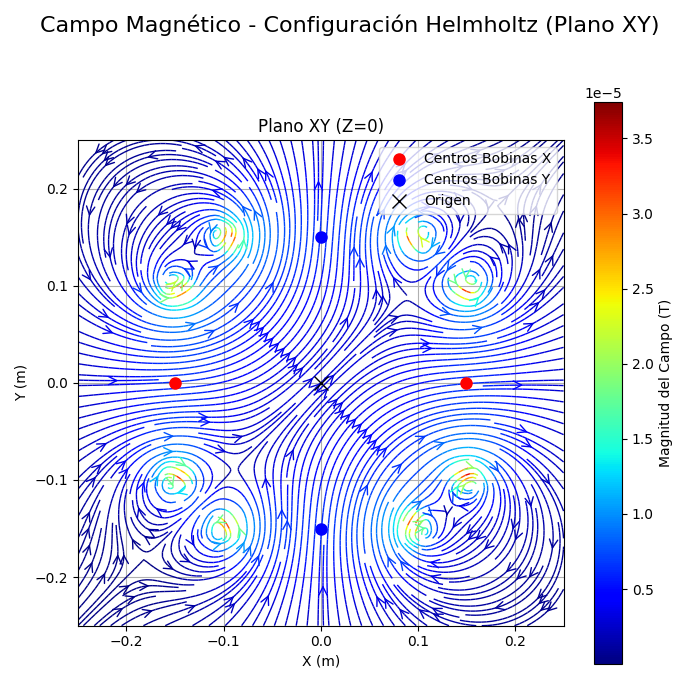
\includegraphics[width=\linewidth]{Sections/Figures/helmholtz_xy_field.png}
        \caption{Bobinas en  Helmholtz.}
        \label{fig:helmholtz_xy_field}
    \end{minipage}
    \hfill
    \begin{minipage}[b]{0.48\textwidth}
        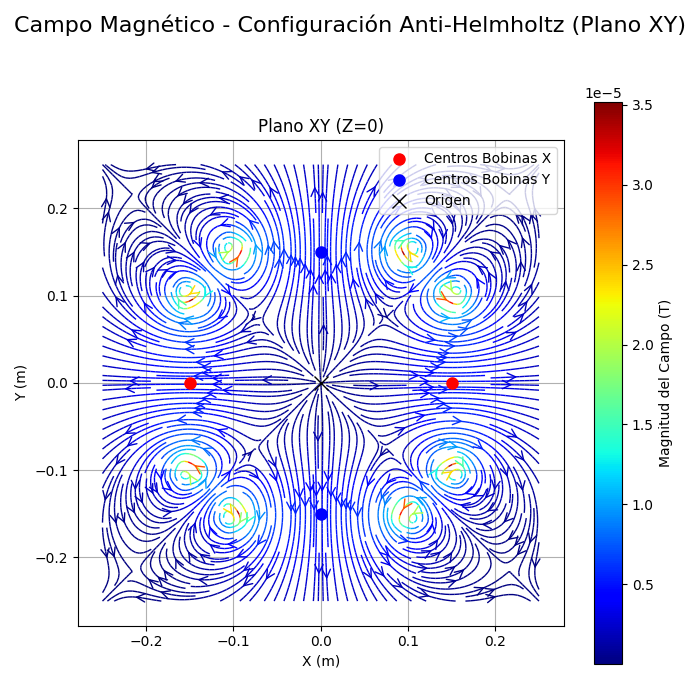
\includegraphics[width=\linewidth]{Sections/Figures/antihelmholtz_xy_field.png}
        \caption{Bobinas en  Anti-Helmholtz.}
        \label{fig:antihelmholtz_xy_field}
    \end{minipage}
    %\caption{Morfología del campo magnético en el plano $x,y$ para las configuraciones Helmholtz y Anti-Helmholtz.}
    \label{fig:campos_bobinas}
\end{figure}

Posteriormente, y dado que se tenía información sobre el comportamiento del campo en cortes del volumen generado por las bobinas, se procedió a graficar el esquema de la simulación basándose en estos campos, como se puede ver en la siguiente gráfica que representa la trayectoria del haz a través de los campos generados.

\begin{figure}[H]
    \centering
    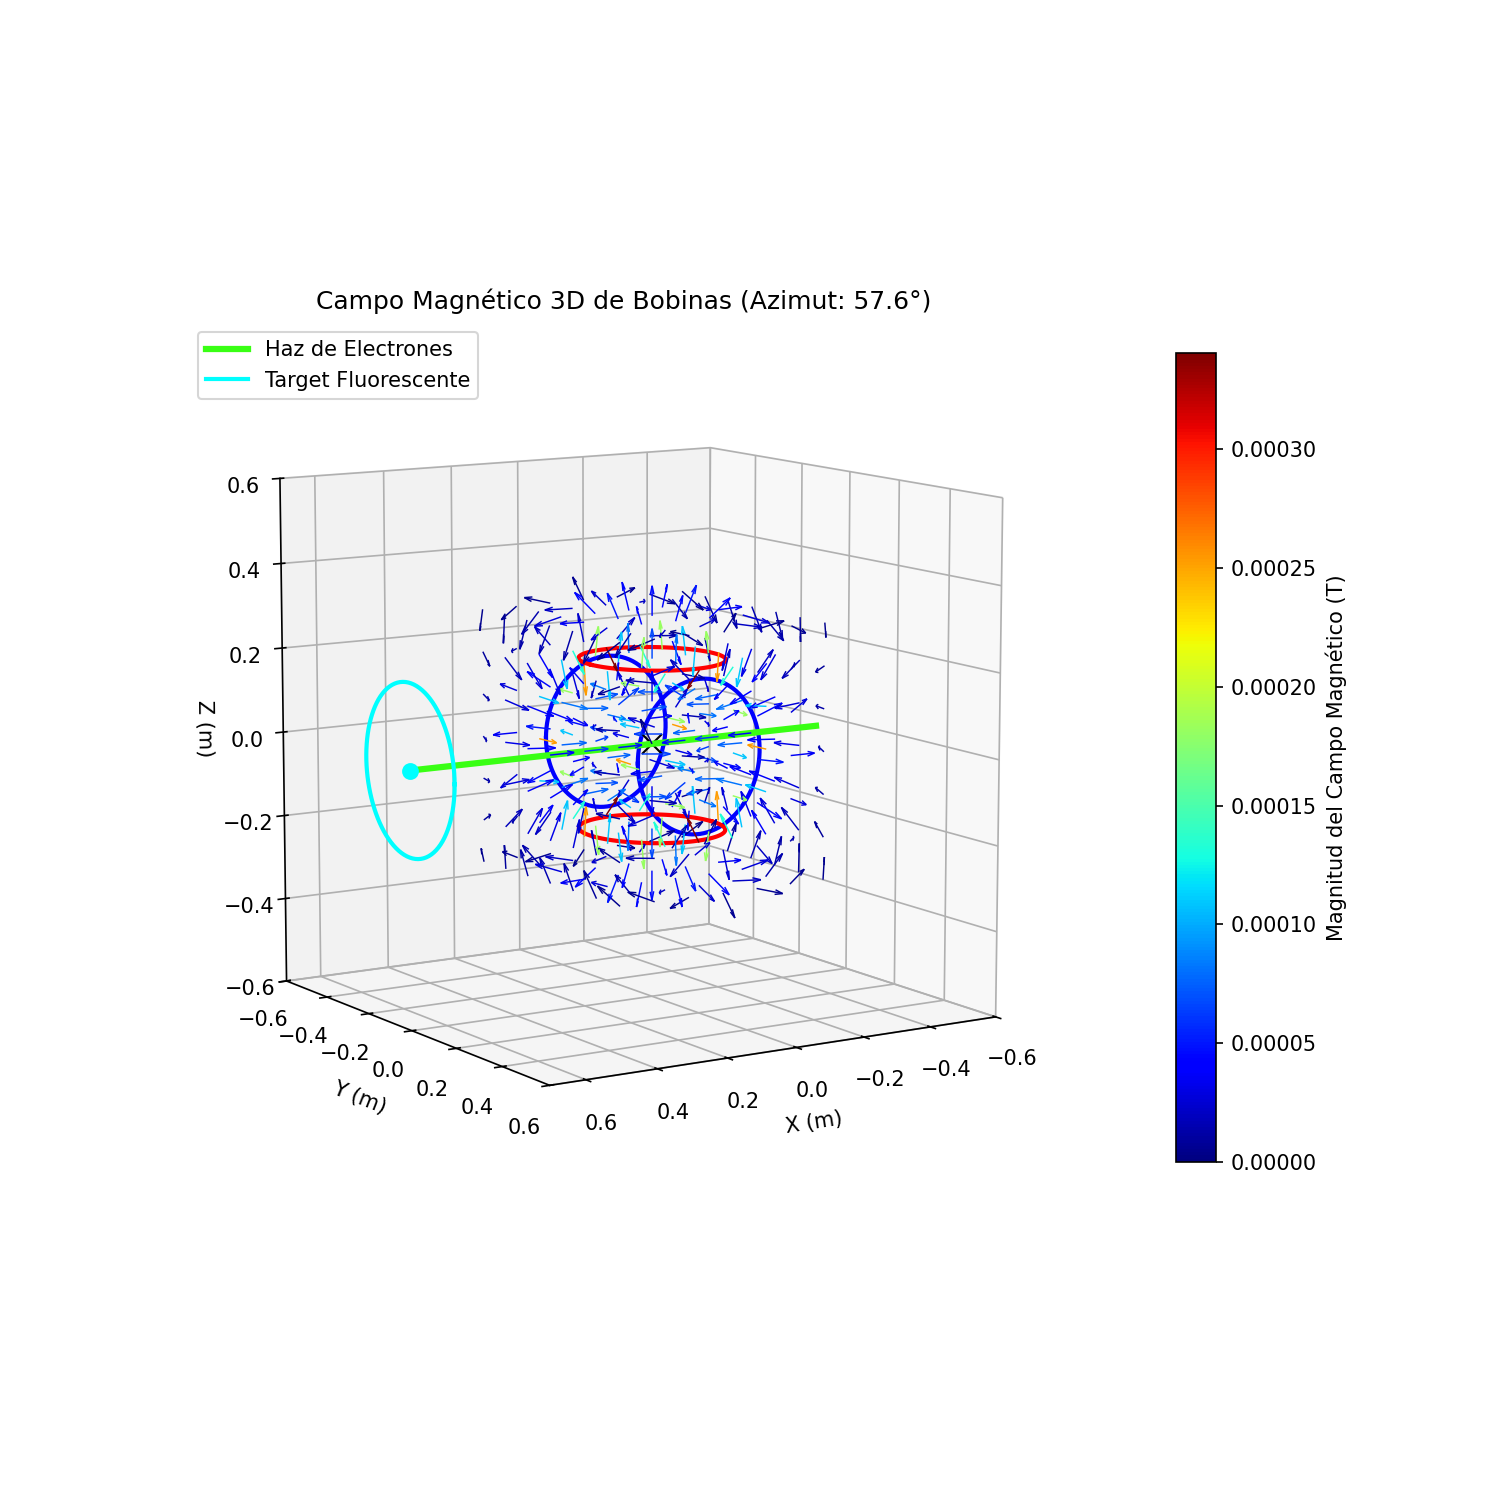
\includegraphics[width=0.8\textwidth]{Sections/Figures/frame_azim_057.6.png}
    \caption{Trayectoria del haz para la simulación.}
    \label{fig:trayectoria_haz_simulacion}
\end{figure}

Finalmente, se realizaron las primeras especulaciones sobre si los \textbf{campos eléctricos inducidos} en el montaje tendrían influencia en la modificación del comportamiento del haz, y si estos deberían considerarse como un factor importante en la simulación. También, tras una investigación sobre el montaje, se pudo observar su similitud con un \textbf{Stern-Gerlach}, donde una característica de su campo magnético es que suelen ser campos no uniformes, generados en muchas ocasiones con sistemas de cuadrupolos. Por lo tanto, se propone que, para optimizar las simulaciones, se contemple la posibilidad de generar los campos con \textbf{dipolos} o \textbf{cuadrupolos}.